\documentclass{sciposter}
\usepackage{lipsum}
\usepackage{epsfig}
\usepackage{amsmath}
\usepackage{amssymb}

% Para Tablas
\usepackage{multicol}
\usepackage{multirow}

% Para gráficas propias
\usepackage{pst-all}
\usepackage{multido,pstricks}

\usepackage{graphicx,url}

% Idioma
\usepackage[spanish]{babel}   

% Codificación
\usepackage[utf8]{inputenc}
%\usepackage{fancybullets}

% Se pueden crear comandos propios de theorems
\newtheorem{Def}{Definici\'on}


% Título del proyecto
\title{Nombre proyecto\\ subt\'itulo}

% Nombre de los autores
\author{Fernando Crema, Alejandro Crema}

% Dirección de la Universidad
\institute 
{Escuela de Computación\\
Facultad de Ciencias \\ 
Universidad Central de Venezuela (UCV)\\
  Av. Paseo Los Ilustres, Los Chaguaramos, Caracas, Venezuela}
  
% Correo electrónico
\email{{fernando.crema,alejandro.crema},{(@ciens.ucv.ve})}

% Logos de universidad y facultad

\rightlogo[1]{logociens}
\leftlogo[1.2]{logo-ucv}

\begin{document}
%define conference poster is presented at (appears as footer)

\conference{{\bf I-2015}, Papers sobre Miner\'ia de Datos, Mayo de 2016, Caracas, Venezuela}

%\LEFTSIDEfootlogo  
% Uncomment to put footer logo on left side, and 
% conference name on right side of footer

% Some examples of caption control (remove % to check result)

%\renewcommand{\algorithmname}{Algoritme} % for Dutch

%\renewcommand{\mastercapstartstyle}[1]{\textit{\textbf{#1}}}
%\renewcommand{\algcapstartstyle}[1]{\textsc{\textbf{#1}}}
%\renewcommand{\algcapbodystyle}{\bfseries}
%\renewcommand{\thealgorithm}{\Roman{algorithm}}

\maketitle

%%% Begin of Multicols-Enviroment
\begin{multicols}{3}

%%% Abstract
\begin{abstract}
% BEGIN MINERIA UCV
Resumen del paper, el problema que resuelve, referencia a Kaggle y breve discusión de los resultados.
% END MINERIA UCV
\end{abstract}

%%% Introduction
\section{Introducci\'on}
% BEGIN MINERIA UCV 
\PARstart{B}{reve} descripción del problema a resolver, importancia seg\'un Kaggle, descripci\'on del dataset.
\emph{\'enfasis de ser requerido}
% END MINERIA UCV

% Ejemplo de citas, dentro va identificador del bibitem
\cite{maragos89:_patter}.
\\ % separar párrafos,
A drawback of the classical definition of pattern spectra is that spatial 
information is not included in a pattern spectrum as shown below.
 In this paper, \emph{spatial pattern spectra} are developed which retain information on the distribution of these details at different scales.
 

\newcommand{\imsize}{0.45\columnwidth}
\begin{figure}
\begin{center}
\begin{tabular}{cc|c|c|c|c|l}
\cline{3-6}
& & \multicolumn{4}{ c| }{Primes} \\ \cline{3-6}
& & 2 & 3 & 5 & 7 \\ \cline{1-6}
\multicolumn{1}{ |c  }{\multirow{2}{*}{Powers} } &
\multicolumn{1}{ |c| }{504} & 3 & 2 & 0 & 1 &     \\ \cline{2-6}
\multicolumn{1}{ |c  }{}                        &
\multicolumn{1}{ |c| }{540} & 2 & 3 & 1 & 0 &     \\ \cline{1-6}
\multicolumn{1}{ |c  }{\multirow{2}{*}{Powers} } &
\multicolumn{1}{ |c| }{gcd} & 2 & 2 & 0 & 0 & min \\ \cline{2-6}
\multicolumn{1}{ |c  }{}                        &
\multicolumn{1}{ |c| }{lcm} & 3 & 3 & 1 & 1 & max \\ \cline{1-6}
\end{tabular}
\end{center}

% Leyenda de cualquier figura, sea tabla o no
\caption{ Parts (a) through (c) show three images consisting of squares of
different sizes;
(d) shows the pattern spectra, denoting the number of foreground pixels 
 removed by openings by reconstruction by $\lambda \times \lambda$ squares. No 
granulometry is capable of separating the patterns, because the only 
differences between the images lie in the distributions of the 
connected components. }\label{fig:blocks} % identificador de la figura
\end{figure}

\section{An\'alisis Exploratorio de Datos}
Dar uma ideia compacta da metodologia ou forma de abordagem da pesquisa, bem como o projeto foi desenvolvido.\\

Let binary images $X$ and $Y$ be defined as a subset of the image domain 
${\mathbf M}\subset {\mathbb Z}^n$ or ${\mathbb R}^n$ (usually $n=2$). 
\begin{Def} % En caso de usar definiciones formales
A binary 
granulometry is a set of operators $\{\alpha_r\}$ with $r$ from some ordered 
set $\Lambda$ (usually $\Lambda \subset {\mathbb R}$ or ${\mathbb Z}$), with 
the following three properties
\begin{align}
% Label a las ecuaciones en caso de ser requerida una cita
   \alpha_r(X) & \subset  X \label{eq:antiext} \\
   X \subset Y & \Rightarrow \alpha_r(X) \subset \alpha_r(Y) 
   \label{eq:increasing} \\
   \alpha_r(\alpha_s(X)) & =  \alpha_{\max(r,s)}(X) \label{eq:idempot},
\end{align}   
for all $r,s \in \Lambda$.
\end{Def}

% Uso de referencias de los labels
Hago referencia a la ecuaci\'on \ref{eq:antiext} de la figura \ref{fig:blocks}

\begin{Def}
The pattern spectrum $s_{\alpha}(X)$ obtained by applying 
granulometry $\{\alpha_r\}$ to a binary image $X$ is defined as
\begin{equation}
    (s_{\alpha}(X))(u) = 
    - \frac{\partial A(\alpha_r(X))}{\partial r}\bigg{\vert}_{r=u}
\end{equation}
in which $A(X)$ is a function denoting the Lebesgue measure in 
${\mathbb R}^n$.
\end{Def} 
In the case of discrete images, and with $r \in \Lambda \subset {\mathbb Z}$, 
this differentiation reduces to
\begin{align}
    (s_{\alpha}(X))(r)  & = \#(\alpha_{r}(X) \setminus \alpha_{r^+}(X)) \\ 
                        & = \#(\alpha_{r}(X)) - \#(\alpha_{r^+}(X)), 
\end{align}
with $r^+ = \min\{ r' \in \Lambda \vert r' > r \}$, and $\#(X)$ the 
numnber of elements of $X$.

The opening transform \cite{Nacken:thesis} $\Omega_X$ of a binary image $X$ 
for a granulometry ${\alpha_r}$ is
\begin{equation}
  \Omega_X(x) = \max\{ r \in \Lambda \vert x \in \alpha_r(X) \}
\end{equation}

The pattern spectrum of a binary image $X$ using granulometry 
$\{\alpha_r\}$ is the histogram of $\Omega_X$ obtained with the same 
size distribution \cite{Nacken:thesis}, disregarding the bin for grey level 0.

% Esta sección va a depender de los proyectos, podría llamarse simplemente PReprocesamiento
\section{Selecci\'on de Variables | Ajuste de Dimensionalidad | Creaci\'on de Variables | Limpieza de datos}
Dar uma ideia compacta da metodologia ou forma de abordagem da pesquisa, bem como o projeto foi desenvolvido.
% Usando subsecciones
\subsection{Limpieza de Datos}
Pattern spectra only retain the amount of detail present at  scale $r$.
This can be amended by computing some parameterization of the spatial 
distribution in an image $\alpha_r(X) \setminus \alpha_{r+}(X)$ as a function of $r$. 

\subsection{Ajuste de Dimensionalidad}

\begin{Def}
Let ${M}(X)$ be some parameterization of the spatial distribution of detail
in the image $X$. The spatial pattern spectrum ${S}_{{M},\alpha}$ is
then defined as
\begin{equation}
  ({S}_{{M},\alpha}(X))(r) = {M}(\alpha_r(X) \setminus \alpha_{r+}(X)).
\end{equation}  
\end{Def}

% Ejemplo de subsecciones
\subsubsection{PCA}
An obvious parameterization of the spatial distribution is through 
the use of moments. Focusing on the case of 2-D binary images, the 
moment $m_{ij}$ of order $ij$ of an image $X$ is given by
\begin{equation}
  m_{ij}(X) = \sum_{(x,y) \in \mathbf X} x^i y^j.
\end{equation}  
The spatial moment spectrum $S_{m_{ij},\alpha}$ of order $ij$ is
\begin{equation}
  (S_{m_{ij},\alpha}(X))(r) = m_{i,j}(\alpha_r(X) \setminus \alpha_{r^+}(X)).
\end{equation}  
For $i=0$ and $j=0$ we obtain the standard pattern spectrum. 
For each $r$, $(S_{m_{ij},\alpha}(X))(r)$ is just the moment of an image, 
therefore, derived parameters such as coordinates of the centre of mass, 
(co-)variances, skewness and kurtosis of the distribution of details at each
scale can be computed easily. We can then define pattern mean
spectra, pattern (co-)variance spectra, pattern kurtosis spectra, etc. The 
pattern mean-$x$ and variance-$x$ spectra 
($S_{\bar x,\alpha}$ and $S_{\sigma(x),\alpha}$) are defined as: 
\begin{align}
  S_{\bar x,\alpha} & = \frac{S_{m_{10},\alpha}} {S_{m_{00},\alpha}} \\
\intertext{and}
   S_{\sigma(x),\alpha} & = \sqrt{\frac{S_{m_{20},\alpha}}
                                 {S_{m_{00},\alpha}} 
                                 - S_{\bar x, \alpha}}.  
 \end{align}
These two are shown in Figures \ref{fig:tauspect} and \ref{fig:binspect}. Note that 
these definitions hold only where $(S_{m_{00},\alpha}(f))(r) \neq 0$. For all 
other values of $r$ they will be defined as zero. Further post-processing can
be done to compute central moments and moment invariant from pattern moment 
spectra \cite{Flusser:Suk:93,Hu:62}. 

% Breve definición del algoritmo escogido por ustedes y razonamiento detrás de esto.
\section{KMedias | Filtrado Colaborativo | M\'aquinas de soporte vectorial | ...}

Verificar os principais resultados obtidos de acordo com os objetivos propostos.\\

Nacken \cite{Nacken:thesis} derived an algorithm for computation
of pattern spectra for granulometries based on openings by discs of increasing
radius for various metrics, using the opening transform. After the
opening transform has been computed, it is straightforward to compute the 
pattern spectrum:
\begin{itemize}
\item Set all elements of array {\tt S} to zero
\item For all $x \in X$ increment {\tt S}[$\Omega_X(x)$] by one. 
\end{itemize}

To compute the pattern \emph{moment} spectrum, the only thing that needs to be
changed is the way {\tt S}[$\Omega_X(x)$] is incremented. As shown in Algorithm
\ref{alg:spect}.

% Ejemplo de uso del paquete Algorithm

\begin{algorithm}
\begin{itemize}
\item Set all elements of array {\tt S} to zero
\item For all $(x,y) \in X$ increment {\tt S}[$\Omega_X(x,y)$] by 
$x^iy^j$. 
\end{itemize}
\caption{ Algorithm for computation of pattern moment
spectrum of order $ij$. \label{alg:spect}}
\end{algorithm}

This algorithm can 
readily be adapted to other granulometries, simply by computing the 
appropriate opening transform.

\begin{figure}
\begin{center}
% Entre corchetes el scale de la imagen
	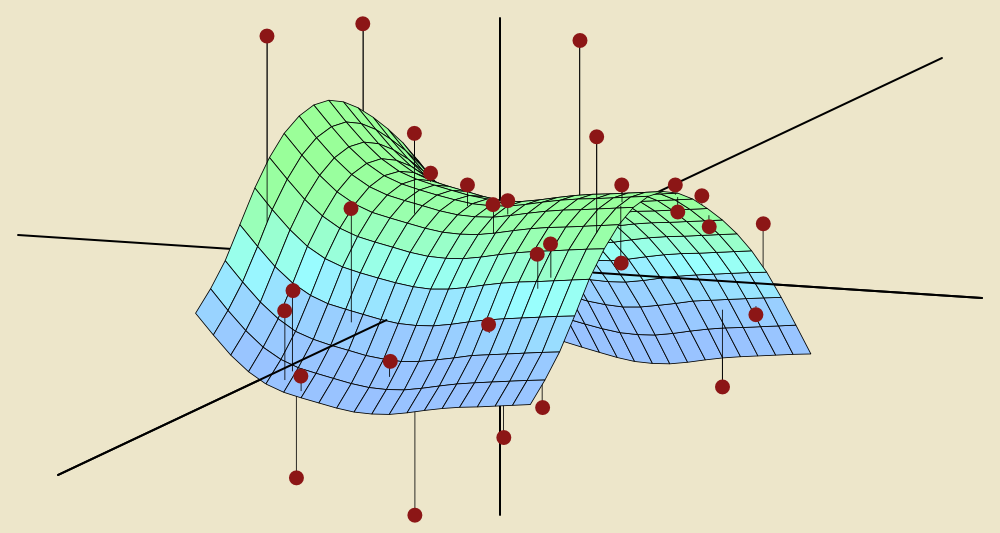
\includegraphics[scale=0.75]{the-mean-machine-learning}
\end{center}
\caption{ \label{fig:tauspect} 
The opening transform using city-block metric: (a) opening transform of
Fig. 1(c); (b) pattern spectrum; (c) pattern variance-$x$; 
(d) variance-$y$ spectra.}
\end{figure}

Este ejemplo es para $\theta = 0$
$$ \text{min } x_1 + x_2 \text{ s.a:} $$ 
$$2 x_1 + x_2 \leq 3$$ 
$$(2 -\theta )x_1 + x_2 \leq 2$$
$$ x_1, x_2 \geq 0 $$

\vfill

\begin{figure}
	\begin{center}
    \scalebox{1.5}{ % escalar pspicture
    \vspace*{25mm} 
      \begin{pspicture}(0,0)(2,3) % Plano desde el punto 0,0 al 2,3
      
      	% Subgrid de fondo
        \psgrid[subgriddiv=1,griddots=10,gridlabels=0pt](0,0)(2,3)
        
        % Polígono interlineado referente a la intersección de las restricciones
        \pspolygon[fillstyle=vlines, linewidth=0.05pt](0,0)(0,2)(1,0)
        
        % Put de una leyenda en la gráfica
        \rput[bl](1,1.5){$\tiny 2 x_1 + x_2 \leq 3$}
        
        % Gráfica de la recta 2-2*x = y
        \psplot[algebraic,plotpoints=2000, linestyle=dashed]{-0.3}{1.35}{2-2*x}
        % Gráfica de la recta 3-2*x = y
        \psplot[algebraic,plotpoints=2000]{-0.3}{1.85}{3-2*x}
        \SpecialCoor
       
       % Graficar ejes, tipo de línea final
       \psaxes{->}(0,0)(-.5,-.5)(2.5,3.8)
       
       % Leyenda de los ejes
        \uput[0](2.5,0){$x1$}
        \uput[90](0,3.7){$x2$}
      \end{pspicture}
      } %end scale box
      \vspace*{15mm} 
	\end{center}
\caption{ \label{fig:binspect} Analizando el impacto de alteraciones sobre restricciones lineales en problemas de programaci\'on lineal. Aplicaci\'on con precios sombra en la econom\'ia.}
\end{figure}

\section{Resultados | Conclusi\'on}

She should not lock the open door
(Run away, run away, run away)
Fullmoon is on the sky and he's not a man anymore
See what became out of her man
 
%%% References

%% Note: use of BibTeX als works!!

\bibliographystyle{plain}
\begin{thebibliography}{1}

\bibitem{Flusser:Suk:93}
J.~Flusser and T.~Suk.
\newblock Pattern recognition by affine moment invariants.
\newblock {\em Pattern Recognition}, 26:167--174, 1993.

\bibitem{Hu:62}
M.~K. Hu.
\newblock Visual pattern recognition by moment invariants.
\newblock {\em IRE Transactions on Information Theory}, IT-8:179--187, 1962.

\bibitem{maragos89:_patter}
P.~Maragos.
\newblock Pattern spectrum and multiscale shape representation.
\newblock {\em IEEE Trans. Patt. Anal. Mach. Intell.}, 11:701--715, 1989.

\bibitem{Meijster:Wilkinson:PAMI}
A.~Meijster and M.~H.~F. Wilkinson.
\newblock A comparison of algorithms for connected set openings and closings.
\newblock {\em IEEE Trans. Patt. Anal. Mach. Intell.}, 24(4):484--494, 2002.

\bibitem{Nacken:thesis}
P.~F.~M. Nacken.
\newblock {\em Image Analysis Methods Based on Hierarchies of Graphs and
  Multi-Scale Mathematical Morphology}.
\newblock PhD thesis, University of Amsterdam, Amsterdam, The Netherlands,
  1994.

\end{thebibliography}

\end{multicols}

\end{document}